%Het eerste hoofdstuk van je thesis.
\chapter{Inleiding}
Deze masterproef behandelt een onderzoek naar het gebruik van camera beveiliging in een slaapomgeving. Met als doel te detecteren wanneer een persoon uit bed stapt en langs welke zijde dit gebeurt. Is het mogelijk om dit te doen? Welke camera kunnen we het best gebruiken? Dit zijn de vragen waar de vooral een antwoord op willen geven. \\
We zijn begonnen met het kijken naar welke verschillende systemen er al zijn en welke technieken interessant kunnen zijn voor ons. We bespreken zo verschillende generaties van surveillance systemen, verschillende types van camera en verschillende methoden om personen te detecteren. Vooral op voorgond achtergrond segmentatie wordt dieper ingegaan. \\
Vervolgens bespereken we een paar experimenten die we gedaan hebben. Onze experimenten zijn in verschillende stappen gebeurd. We beginnen zeer eenvoudig met het opslaan en ophalen van afbeeldingen. Vervolgens gaan we verder met de effectieve persoon detectie. Nadat de persoon gedetecteerd wordt, gaan we verder met de detecte van de zijde waarlangs er uit bed gestapt wordt. Om dit te kunnen bereiken maken we gebruik van temporeel verschil. Als allerlaatste hebben we ons algoritme toegepast op live beelden. \\
Uit de kleine experimenten hebben we elk keer onze belsuiten getrokken en nieuwe experimenten uitgevoerd. Dit tot we uiteindelijk aan het algemeen besluit komen. 

\chapter{Literatuurstudie}
In dit hoofdstuk gaan we nakijken of er reeds werken geschreven zijn die voor ons toepasselijk zijn. Voor we beginnen aan het maken van het project, gaan we eerst op zoek naar reeds bestaande systemen, deze worden beschreven in sectie \ref{refRBS}, we bekijken welke types van surveillance systemen er bestaan en bestuderen welke eventueel interessant kunnen zijn voor ons project in sectie \ref{refTVS}, dit wordt gevolgd door sectie \ref{refTVC}, deze omvat  een beschrijving van verschillende types van camera's. Als laatste deel van de literatuurstudie bestuderen we reeds bestaande algoritmes voor persoonsherkenning in sectie \ref{refAVPH}. Dit hoofdstuk wordt afgesloten in sectie \ref{refLBe} met een besluit over de literatuurstudie.

\section{Reeds bestaande systemen}
\label{refRBS}
Het eerste wat we onderzochten was of er al gelijkaardige systemen bestonden. Onze zoekacties op het internet leverden aanvankelijk geen resultaten op. Al blijkt dat er in bijvoorbeeld de slaapkliniek van A.Z. Monica ook gewerkt word met een infraroodcamera. Daarover was verder geen informatie te vinden. Gedurende de rest van het jaar bleven we verder zoeken naar soort gelijke systemen, omdat de mogelijkheid altijd bestaat dat er nieuwe informatie beschikbaar komt.

\section{Types van surveillance systemen}
\label{refTVS}
In dit deel van de literatuurstudie gaan we onderzoeken welke types van surveillance systemen er zijn. We gaan eveneens bestuderen welke types zinvol zijn voor ons project. Waarom zouden we werken met camerabeveiliging? Je zou ook een systeem kunnen maken door gebruik te maken van druk sensoren in een mat naast het bed, of onder de matras zelf. Het voordeel van camera gestuurde surveillance is dat we kunnen zien wat er op het moment zelf gebeurt, maar dat we ook achteraf gebeurde incidenten kunnen reconstrueren. Het nadeel van camera gestuurde surveillance is dat we incidenten moeten kunnen identificeren en herkennen op het  moment dat ze gebeuren \cite{bibVTC3}. Er zijn drie verschillende generaties van surveillance systemen. De eerste generatie van surveillance systeem dat we gaan bestuderen is het traditionele surveillance systeem, meer informatie hierover is terug te vinden in sectie \ref{refTST}, daarna gaan we verder met de tweede generatie van surveillance systemen in sectie \ref{refTGS}, dit wordt gevolgd in sectie \ref{refINS} door een bespreking van de intelligente surveillance systemen.  Een surveillance systeem kan door middel van verschillende parameters ge\"evalueerd worden. Bijvoorbeeld door een studie van de tijdsvertraging tussen het voorvallen van een gebeurtenis en de detectie. Er wordt momenteel ook nog steeds onderzoek gedaan op gebied van de verschillende types van camera gestuurde surveillance.

\subsection{Traditionele surveillance systemen}
\label{refTST}
De traditionele surveillance systemen zijn de eerste van drie generaties van surveillance systemen. Ze maken gebruik van analoge technologie doorheen het volledige systeem, dit is een van de grootste nadelen van dit type van systeem \cite{bibIPC2}.  Analoge camera's maken in dit type van systeem, de beelden van de sc\`ene. De signalen worden verzonden over communicatielijnen naar de  toestellen, waar de data weergegeven en opgeslagen worden \cite{bibVTC2}. In een traditioneel surveillance systeem is de kwaliteit en de kost recht evenredig met het aantal gebruikte camera's. Voor een grote omgeving, worden er voor een systeem meerdere camera's gebruikt, om een hele omgeving te bestuderen. Bijgevolg wordt er een grote hoeveelheid aan data verzameld die achteraf verwerkt moet worden.  In onze toepassing, moet er enkel het bed bestudeerd worden. Hierdoor hebben wij een kleine omgeving en volstaat het om \'e\'e camera te hebben voor de detectie van het patienten gedrag. Indien er ook valdetectie gedaan wordt, zijn er  twee camera's nodig om een dieptebeeld te cre\"eren. Meestal is er een persoon nodig die altijd naar de monitor kijkt \cite{bibVTC}. Omdat wij meerdere pati\"enten in het oog willen houden, is dit voor ons niet mogelijk. In sommige gevallen geeft deze methode zeer goede resultaten.

\subsection{Tweede generatie surveillance systemen}
\label{refTGS}
In de tweede generatie van surveillance systemen wordt er gebruik gemaakt van digitale componenten. De overstap van analoge naar digitale technologie is nog niet compleet. Er wordt een combinatie van beide technologie\"en. Automatische visuele surveillance wordt hier mogelijk door een combinatie van computer visuele technologie met Closed Circuit Television (CCTV) systemen \cite{bibIPC2}. Hierdoor is de detectie van gebeurtenissen eenvoudiger voor de gebruiker. Deze dient eens het programma geschreven is en de detecties automatisch doet, zelf niets meer te doen. De alarmtijd wordt korter. Doordat een computer de detectie doet, en niet meer een persoon, kunnen we elke kamer uitrusten met een surveillance systeem. Bij traditionele surveillance systemen zou dit gelijk zijn als voor elke kamer een persoon te betalen om de kamers te bewaken. Door de automatisatie kunnen  we meerdere kamers in het oog gehouden worden. De kwaliteit van het surveillance systeem is beter \cite{bibVTC2}, dit doordat de reactie tijd hoger is. E\'en van de nadelen is dat je algoritmes nodig hebt voor de gedragsanalyses \cite{bibIPC2}. Het ontwikkelen van deze gedragsanalyses gaat tijden de ontwikkel fase veel tijd in beslag nemen. Eens deze ontwikkelt zijn en goede resultaten hebben, gaan zij bijdragen tot de betere resultaten van het surveillance systeem ten opzichte van de traditionele systemen. Het ontwikkelen van dergelijk gedragsanalyse omvat het grootste deel van het onderzoek dat in dit werk gedaan wordt. 

\subsection{Intelligente surveillance}
\label{refINS}
Dit is het derde en eveneens laatst generatie van beeld gestuurde surveillance systemen. Hier is de overgang naar een volledig digitaal systeem compleet\cite{bibVTC2}. Daarom wordt het vaak een intelligent surveillance systeem genoemd. Het kan automatisch zeer grote regio's verwerken. Een groot voordeel is dat er verschillende soorten van sensoren kunnen gecombineerd worden waardoor er zeer veel informatie beschikbaar is. Het opzetten van een dergelijk systeem is moeilijker dan het opzetten bij de voorgaande generaties. men moet het systeem trainen om de incidenten te detecteren. Men  kan dit zowel manueel als computergestuurd doen. Hoe meer data je nodig hebt om het systeem te trainen, hoe meer men het proces moet automatiseren \cite{bibVTS}. Het verwerken van de beelden die gemaakt worden gebeurt in verschillende stappen.  Welke stappen deze zijn en in welke volgorde ze gebeuren, zijn te zien in figuur \ref{imgVTS} \cite{bibIPC2}.
\begin{figure}[hbp]
	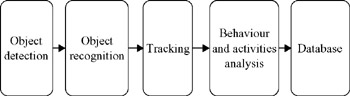
\includegraphics[scale=0.8]{FlowSurveillance}
	\caption{Traditionele flow voor het verwerken van beelden in een surveillance systeem}
	\label{imgVTS}
\end{figure}

\section{Verschillende types van camera's}
\label{refTVC}
In het tweede deel van de literatuurstudie doen we onderzoek naar verschillende types van camera's. En bekijken of deze al dan niet bruikbaar zijn voor ons project. Waarom zijn niet alle camera's geschikt? Aangezien het project gaat over het bestuderen van het slaapgedrag van pati\"enten, gaan onze beelden gemaakt worden in een donkere omgeving. Hierdoor zal er met sommige camera's bijna niets te zien zijn. Het eerste type van camera dat we bespreken is de infraroodcamera in sectie \ref{refIRC}, dit type camera werkt met warmte-verschillen. Een ander type van camera dat we mogelijk ook kunnen gebruiken is  de night vision camera, deze wordt besproken in sectie \ref{refNVC}. Dit is een type van camera speciaal ontworpen om in donkere omgevingen te werken. Een derde mogelijk type van camera wordt besproken in sectie \ref{refIPZ}, namelijk een IP-camera. Nadat we de werking van de IP camera bekijken, gaan we deze uitbereiden met PTZ-camera's, dit is terug te vinden in sectie \ref{refIPC2}.

\subsection{Infraroodcamera}
\label{refIRC}
We hebben het vermoeden dat de infrarood (IR) camera interessant kan zijn omdat deze warmte-verschillen weergeeft. In tegenstelling tot camera's die opereren in de zichtbare band van het spectrum werkt de IR camera  een lange golflengte (8-12 $\mu$m). Een IR sensor gaat de elektromagnetische golven, die zich in het spectrum van de  camera bevinden, uitgestraald door objecten in een sc\`ene, als een thermische afbeelding weergeven,. Waarvan elke pixelwaarde een temperatuur voorstelt \cite{bibIRC2}. We gaan dus de persoon, indien deze zich binnen het bereik van de camera bevindt waarnemen, ongeacht of het dag of nacht is. Dit komt doordat de temperatuur van een pati\"ent, normaal gezien, hoger is als deze van de omgeving \cite{bibIRC3}.
De eerste bedenkingen hierbij zijn of het mogelijk is om een persoon te detecteren als deze gebruik maakt van een elektrisch warmtedeken. Verder gaat het bed ook opwarmen. We moeten dus ook bekijken of er geen valse persoonsdetecties gebeuren op de warme lakens als de persoon in kwestie niet meer in het bed ligt. Verder is de camera ongevoelig voor lichtinval. Hierdoor gaat het bijvoorbeeld geen schaduwen maar ook geen kleuren van kleding waarnemen. Een voordeel van dit type camera is dat een persoon al onherkenbaar is op de beelden. Dit is \'e\'en van de vereisten van ons systeem. Een probleem doet zich voor wanneer een pati\"ent naar de badkamer gaat en er vervolgens een ander persoon de kamer binnen komt. Dit  zal in de beelden zeer weinig verschil veroorzaken en er kunnen valse detecties gebeuren.  Een ander probleem dat opduikt is dat er kringen verschijnen rond gebieden met een zeer hoge of zeer lage temperatuur \cite{bibIRC4}. De sterkte en grootte van deze kringen is afhankelijk van het actuele temperatuurverschil tussen de persoon en de omgeving, en de contrast/gain instellingen van de camera \cite{bibBET6}. Een van de grote voordelen is de uitzonderlijk lage signal to noise ratio (SNR). In het begin werd de IR camera voornamelijk in militaire toepassingen gebruikt. Door de daling van de prijs van een infrarood camera wordt deze tegenwoordig steeds vaker gebruikt in verschillende toepassingen zoals bijvoorbeeld industri\"ele inspectie, door de politie en ook in surveillance systemen\cite{bibBET6}. Op het internet zijn er ook veel verschillende manieren te vinden om van een oud fototoestel zelf een infraroodcamera te maken. Al blijken deze niet altijd goed te werken.
Dankzij de vele toepassingen en de dalende prijs, zijn er ook veel bedrijven die met IR camera's op de markt komen die door ons gebruikt kunnen worden. Hieronder is een lijst te vinden met een paar voorbeelden van dergelijke bedrijven.
\begin{itemize}
	\item Heimann Sensor
	\item Excelitas met CoolEye sensor
	\item Panasonic in samenwerking met AS electronic
	\item Infinitegra
	\item Seek Thermal
\end{itemize}

\subsection{Night vision camera}
\label{refNVC}
Een ander type van camera dat ook mogelijkheden biedt, is een night vision camera. Een afbeelding van zo een camera, is te vinden in figuur \ref{imgNVC}\cite{bibNVC}. Het nadeel van deze camera is dat de persoon wel herkenbaar is op de beelden die rechtstreeks komen van de camera. Terwijl in de vereisten van ons systeem staat dat de persoon onherkenbaar moet zijn op de beelden. Dit kan natuurlijk achteraf door middel van beeldverwerking aangepast worden, door bijvoorbeeld een masker te cre\"eren door huidsegmentatie toe te passen op de beelden. Deze camera's zijn duurder dan de eerste besproken IR camera's in sectie \ref{refIRC}.
\begin{figure}[hbp]
	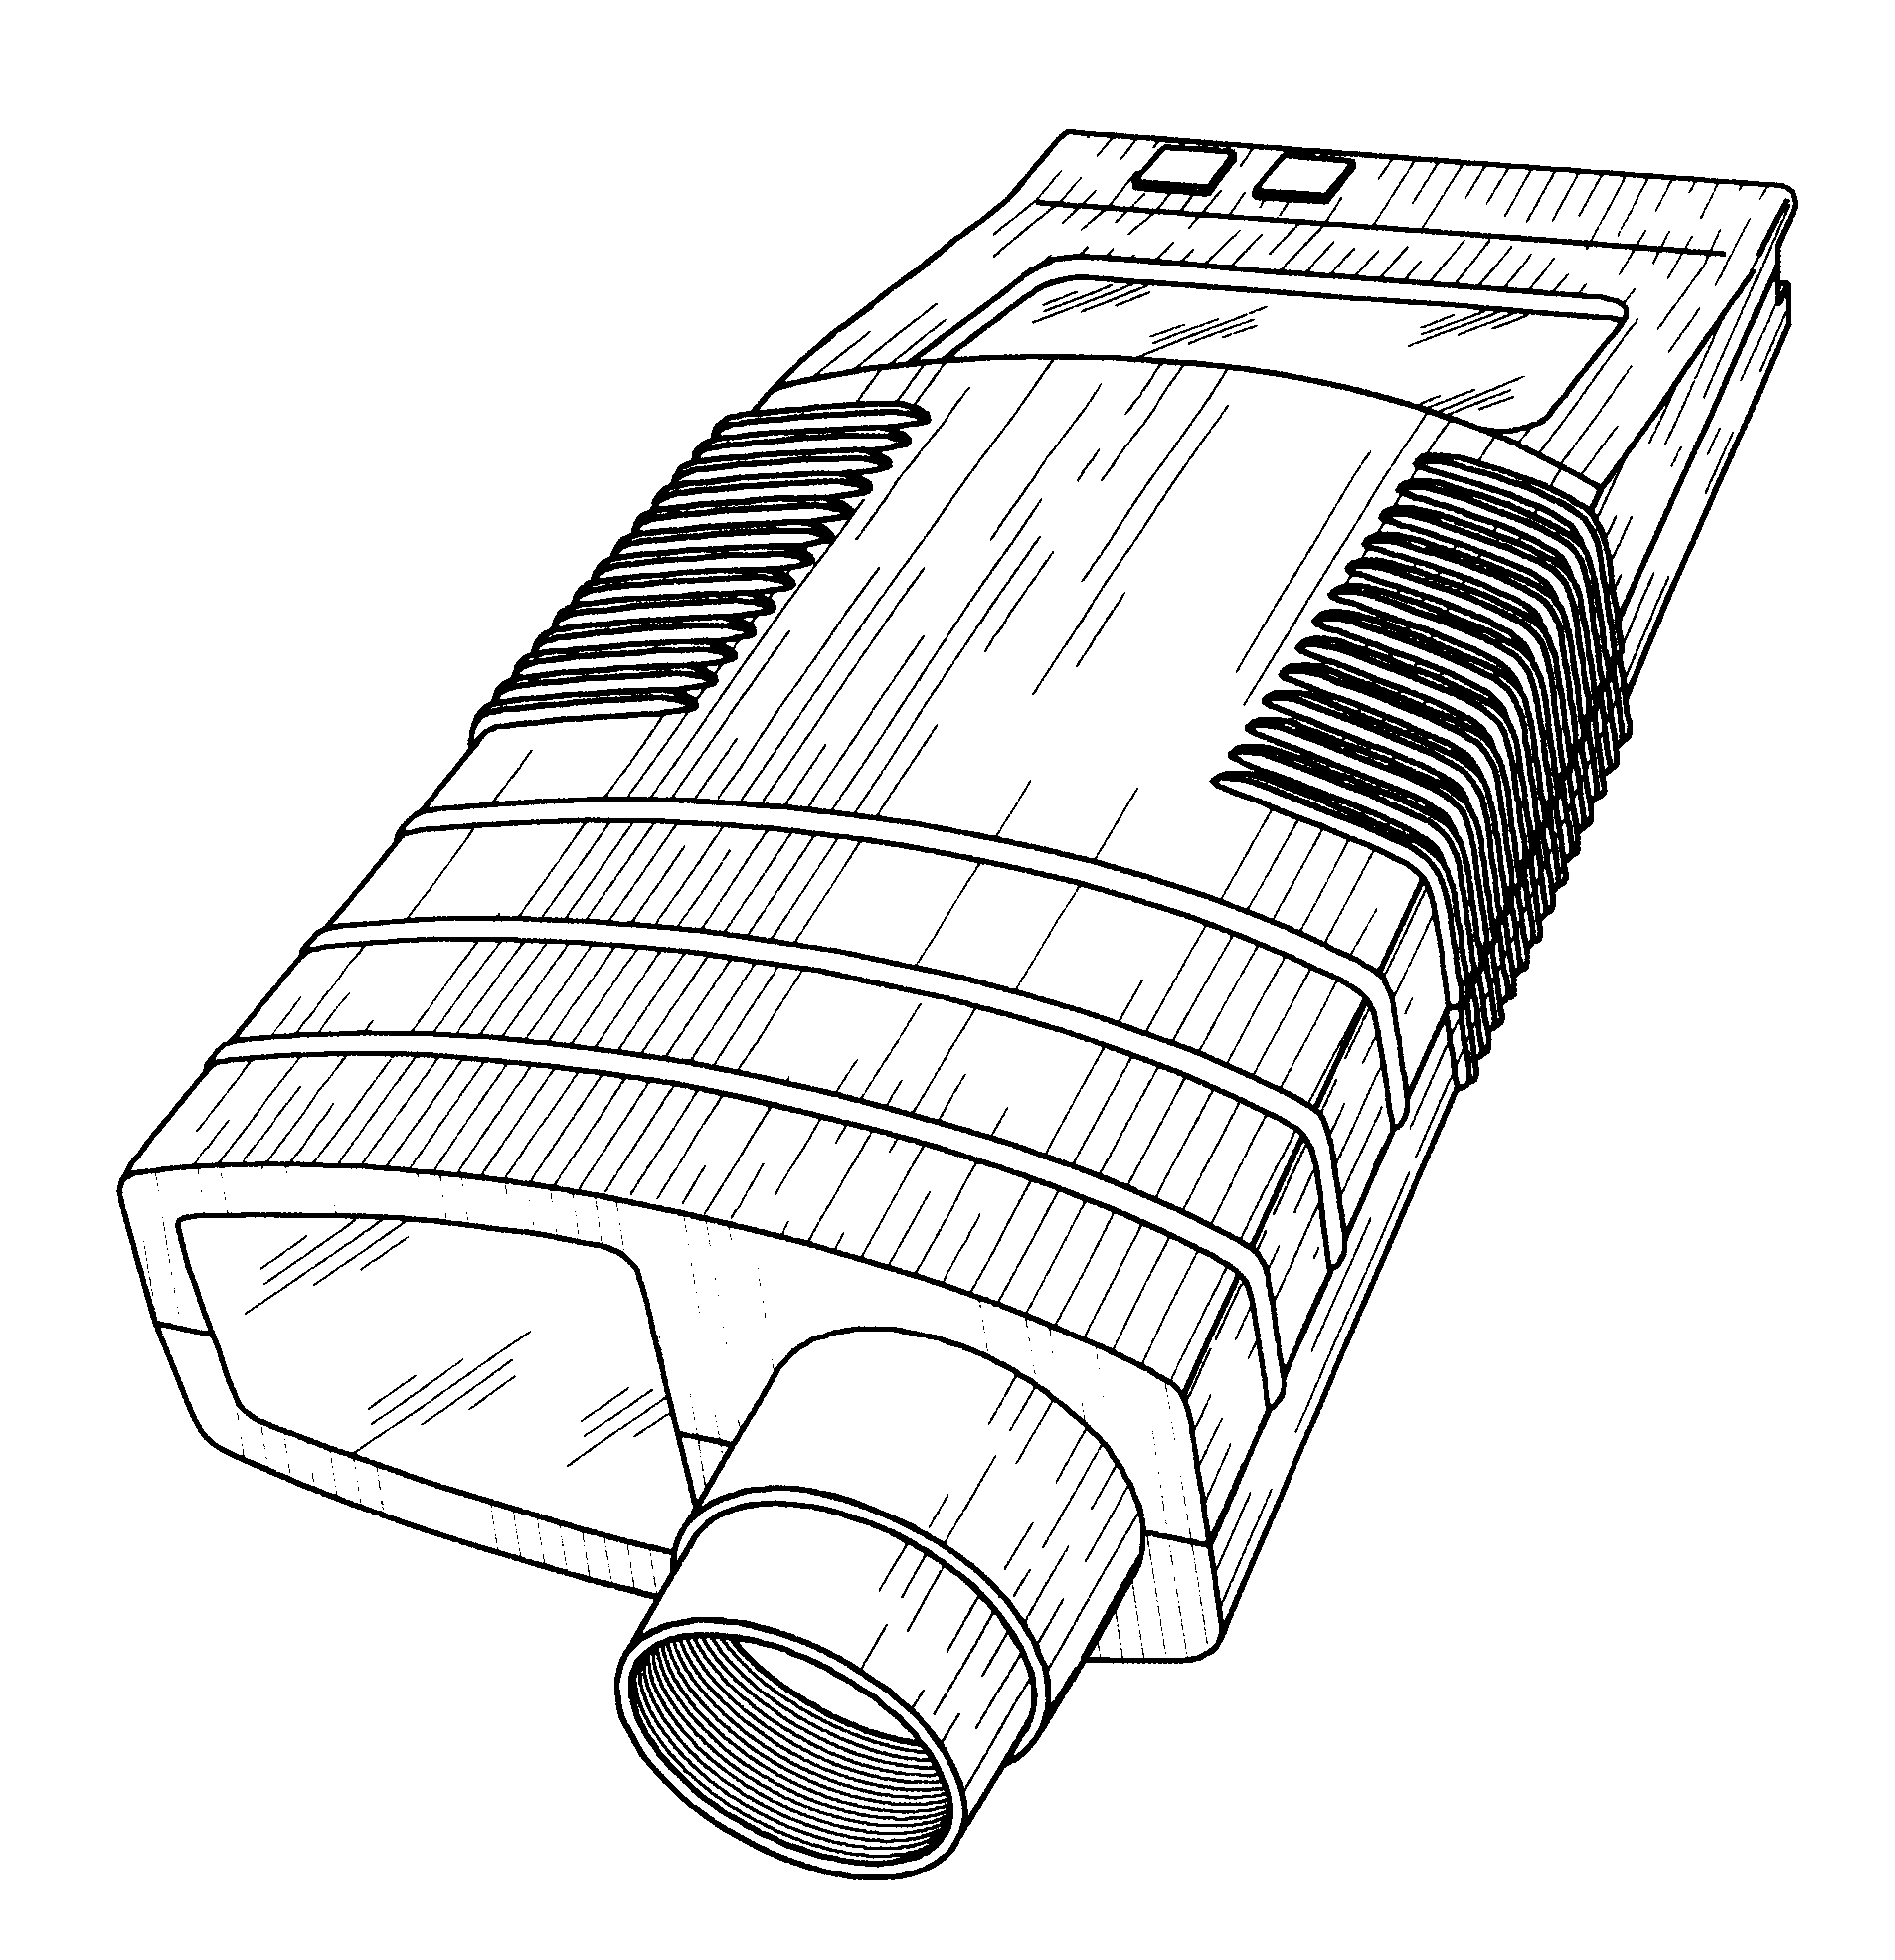
\includegraphics[scale=0.075]{NightVisionCamera}
	\caption{Afbeelding van een night vision camera}
	\label{imgNVC}
\end{figure}

\subsection{IP camera}
\label{refIPC}
IP staat voor Internet Protocol. Het is een camera voorzien van de mogelijkheid om verbinding te maken met het internet. De camera functioneert op je computer netwerk. De camera wordt aangesloten aan een router, switch of draadloos netwerk.  De camera combineert de traditionele camera en netwerk video technologie. De IP camera kan live video comprimeren in de camera zelf wordt de video data omgezet naar digitale data, die al voor een deel verwerkt is. Enkel een abstracte beschrijving van het beeld wordt verder gestuurd \cite{bibIPC3}.  De data wordt over het internet verzonden zonder daarvoor een computer te gebruiken. De basis architectuur van de IP camera ziet u in figuur \ref{imgIPC} \cite{bibVTC2}.
\begin{figure}[hbp]
	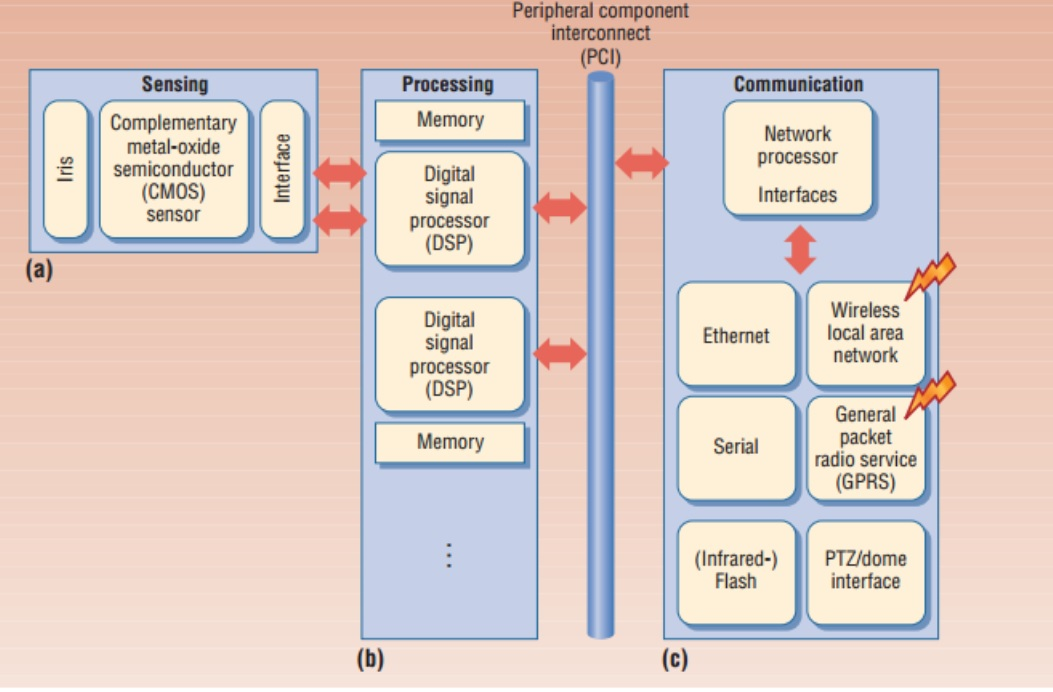
\includegraphics[scale=0.55]{ArchitectuurIPCamera}
	\caption{Hardware architectuur IP camera bestaande uit 3 delen: (a) Sensor eenheid, (b) Verwerkings eenheid, (c) Communicatie eenheid.}
	\label{imgIPC}
\end{figure}
De camera is opgebouwd uit drie delen. Het eerste deel is de sensor eenheid, deze bestaat meestal uit een zeer dynamische monochrome complimentary metal-oxide semiconductor (CMOS) afbeelding sensor. In sommige gevallen komen hier ook andere sensoren bij. Het tweede deel van de architectuur, is de afhandelingseenheid. Deze bestaat uit Digital Signal Processor (DSP). Zij bieden een goede compromis tussen prestatie, vermogen verbruik en flexibiliteit.  De verbinding met de netwerk processor wordt tot stand gebracht door Perpiheral Component Interconnect (PCI) bus. De netwerk processor gaat zorgen voor de interconnectie tussen de communicatie- en afhandelingseenheden. Indien er nog verdere afhandeling van de beelden nodig is, zijn er een paar vaste stappen: object detectie en herkenning, volgen, gedragsanalyse en ophalen van de data \cite{bibIPC2}. Er zijn verschillende soorten van IP camera's, je hebt er voor gebruikt binnen en buiten, of speciaal uitgerust voor gebruik 's nachts, al dan niet met infrarood. De camera die wij nodig hebben is er \'e\'en voor binnen, die uitgerust is voor 's nachts. Het prijskaartje hiervan kan al snel oplopen tot een paar honderden euro's. Dit type camera wordt vooral gebruikt voor bewakingssystemen, ook in de medische sector, verder vormen ze ook de kern van surveillance in de toekomst.

\subsection{IP en PTZ camera's}
\label{refIPC2}
De uitbereiding van twee IP camera's met een PTZ camera wordt gedaan, om een dieptebeeld te kunnen vormen. Dit is nodig voor een mogelijke uitbereiding van dit onderzoek, namelijk de detectie van een pati\"ent die uit bed valt.  We beginnen met twee IP camera's om de positie en locatie van een persoon te bepalen, deze worden automatisch uit de beelden van de camera's gehaald. De positie en locatie worden dan doorgestuurd naar een Pan-Tilt-Zoom (PTZ) camera. De camera wijst en zoomt naar de juiste locatie in de ruimte. In ons geval dus naar de pati\"ent. Hierdoor wordt van de persoon een goed kwalitatief beeld gevormd. Het ontwerp van zo een systeem is te zien in figuur \ref{imgIPC2} \cite{bibIPC}. De grootste moeilijkheid bij dergelijke constructie is dat je de goniometrische relatie tussen de verschillende camera's moet kennen. Om ervoor te zorgen dat dit in orde is kan je een kalibratie doen. Het is door deze goniometrische relatie dat de co\"ordinaten bepaald worden waar de PTZ camera's op gaan inzoomen. \cite{bibVTC3}. Een groot nadeel van deze opstelling is natuurlijk de extra kost van een IP camera en een PTZ camera. We moeten ook de afweging maken of het verkrijgen van een nauwkeuriger beeld van de pati\"ent door de PTZ camera het maken van de extra kost waard is. Anders zouden wij ook de opstelling zonder PTZ camera kunnen gebruiken om de diepte te kunnen bepalen voor de valdetectie.
\begin{figure}[hbp]
	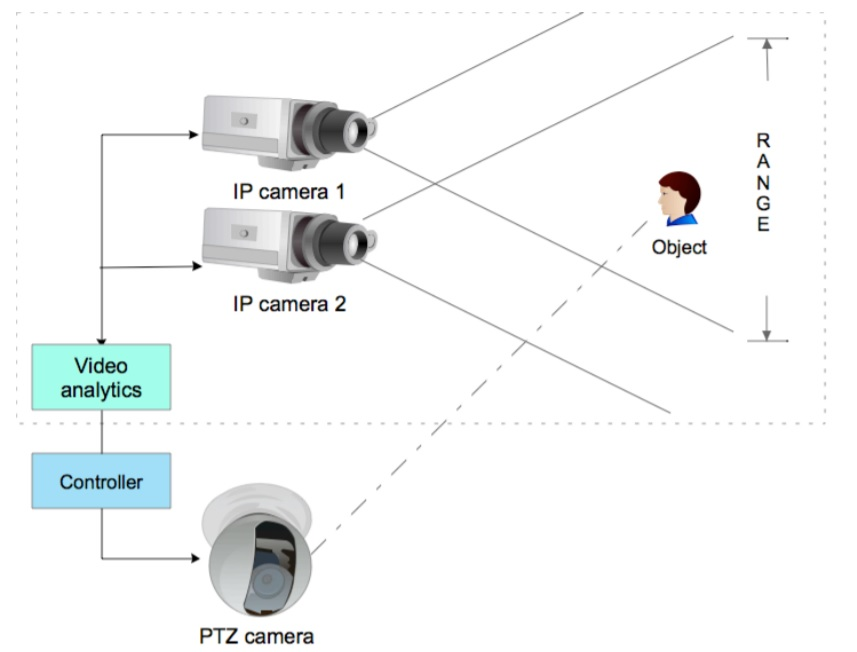
\includegraphics[scale=0.5]{IPPTZCamera}
	\caption{Systeem ontwerp met twee IP camera's en een PTZ camera}
	\label{imgIPC2}
\end{figure}

\section{Algoritmes voor persoonsherkenning}
\label{refAVPH}
In dit hoofdstuk bespreken we algoritmes voor persoonsherkenning. Deze hebben we nodig om de pati\"ent uit het frame te halen. Er zijn veel verschillende methodes ontwikkeld. In dit hoofdstuk bespreken we er een paar die we onderzocht hebben.  De eerste techniek is het thresholden van kleuren, alle informatie hierover is te vinden in sectie \ref{refTVK}. Hierna wordt background estimation techniek of voorgrond- achtergrondsegmentatie besproken in sectie \ref{refBET}. Deze techniek vaak gebruikt voor het volgen van mensen en bewegingen. Ze zijn vooral bruikbaar bij een stationaire camera \cite{bibIRC}. Aangezien wij in ons onderzoek een stationaire camera hebben, is dit voor ons een zeer interessante techniek. Een nadeel is dat elke vorm van verandering wordt gedetecteerd als de pati\"ent, waardoor het soms kan lijken dat er meerdere pati\"enten in een kamer zijn en er dus valse detecties kunnen optreden. Een oplossing hiervoor is een vorm gebaseerde benadering, die we zullen bespreken in sectie \ref{refVBB} \cite{bibIRC}. In de meeste gevallen worden verschillende van deze methoden gecombineerd op uiteindelijk goede resultaten te krijgen. 

\subsection{Thresholden van kleuren}
\label{refTVK}
Dit algoritme is gebaseerd op de kleuren dat een object heeft op de beelden. Deze techniek kan voor veel applicaties gebruikt worden, zoals het detecteren van personen, zoals ook onze bedoeling is, of bijvoorbeeld het detecteren van het rood uit verkeersborden. Deze methode is pixel gebaseerd, voor elke pixel wordt de kleurwaarde vergeleken met een regio in het kleurenspectrum. Zo kunnen we in onze toepassing pixel per pixel zien of het al dan niet gaat om een persoon \cite{bibTHK}. Er zijn verschillende systemen om kleuren te benoemen, bijvoorbeeld:
\begin{description}
	\item[RGB] Rood Groen en Blauw
	\item [CMY] Cyaan, Magentha and Yellow: De primaire kleuren van de kleurpigmenten
	\item [HSI] Hue, Saturation and Intensity
	\item [YUV] Y = helderheid en UV chrominantie (kleurcomponenten)
\end{description}
We kunnen in het algoritme spelen met de verschillende systemen, zo kunnen we zien waar de persoon het makkelijkst uit het beeld te halen is. Indien we dit algoritme gebruiken, gaan we gebruik maken van OpenCV. Om de ruis achteraf te gaan verminderen, kunnen we erosie en dillatie, een median filter of een andere methode gebruiken. 
 
\subsubsection{Jones and Rehg}
Ze maakten een model op basis van internet afbeeldingen. Ze onderzochten welke kleuren in welke verhoudingen voorkomen in de huidskleur op de verschillende afbeeldingen. Nadat dit model af was hebben ze een ander model toegevoegd dat huid- en niet huidafbeeldingen scheidt. Ze maakten een huidhistogram waarin ze de kleur verhoudingen van huid gelabelde afbeeldingen staken, ze maakten ook een niet-huidhistogram waarin ze de kleur verhoudingen van niet-huid gelabelde afbeeldingen staken. Dankzij deze histogrammen kan men de kans berekenen dat huid voorkomt in een bepaalde pixel \cite{bibTHK}. Doordat wij onze beelden 's nachts maken en er dan weinig lichtinval is, gaan in onze toepassing, de kleurwaarden anders zijn. Verder gaan wij ook op beelden gemaakt met een infraroodcamera geen huidskleur zien. Bijgevolg is dit dus een techniek die niet van toepassing is voor ons onderzoek. 

\subsubsection{Dawod et al.}
Dit model staat ook gekend als het RGB-H-CbCr model. Dit is een pixel gebaseerde methode. De beelden worden bekeken in drie verschillende kleurruimtes. De eerste kleurruimte is het RGB domein. Vervolgens wordt gebruik gemaakt van het HSV-domein en als laatste het YUV-domein. In elke kleurruimte wordt er beslist of een pixel al dan niet huid is. Achteraf worden de drie ruimtes samengevoegd en besloten of een pixel al dan niet huid is, de huidpixels moeten een aaneensluitende regio vormen. \cite{bibTHK}.

\subsection{Voorgrond/achtergrond segmentatie}
\label{refBET}
Deze techniek wordt ook background estimatation genoemd, een versie hiervan hebben we gebruikt tijdens een labo in het masterjaar. De techniek is gebaseerd op het feit dat een beeld bestaat uit een achtergrond die niet verandert en een voorgrond die dus alle bewegende en veranderde delen bevat. Eens de achtergrond bepaald is, wordt deze van de nieuwe frame afgetrokken. De verschilwaarde wordt dan vergeleken met een drempelwaarde. Als de verschilwaarde groter is dan de drempelwaarde, wordt ze op de resultaten afbeelding op 1 gezet, indien ze kleiner is dan de  drempelwaarde wordt die pixel op de resultaten afbeelding 0. Ze krijg je een binair beeld. Dit kan je zien op figuur \ref{imgVAS}.\cite{bibVAS}.

\begin{figure}[hbp]
	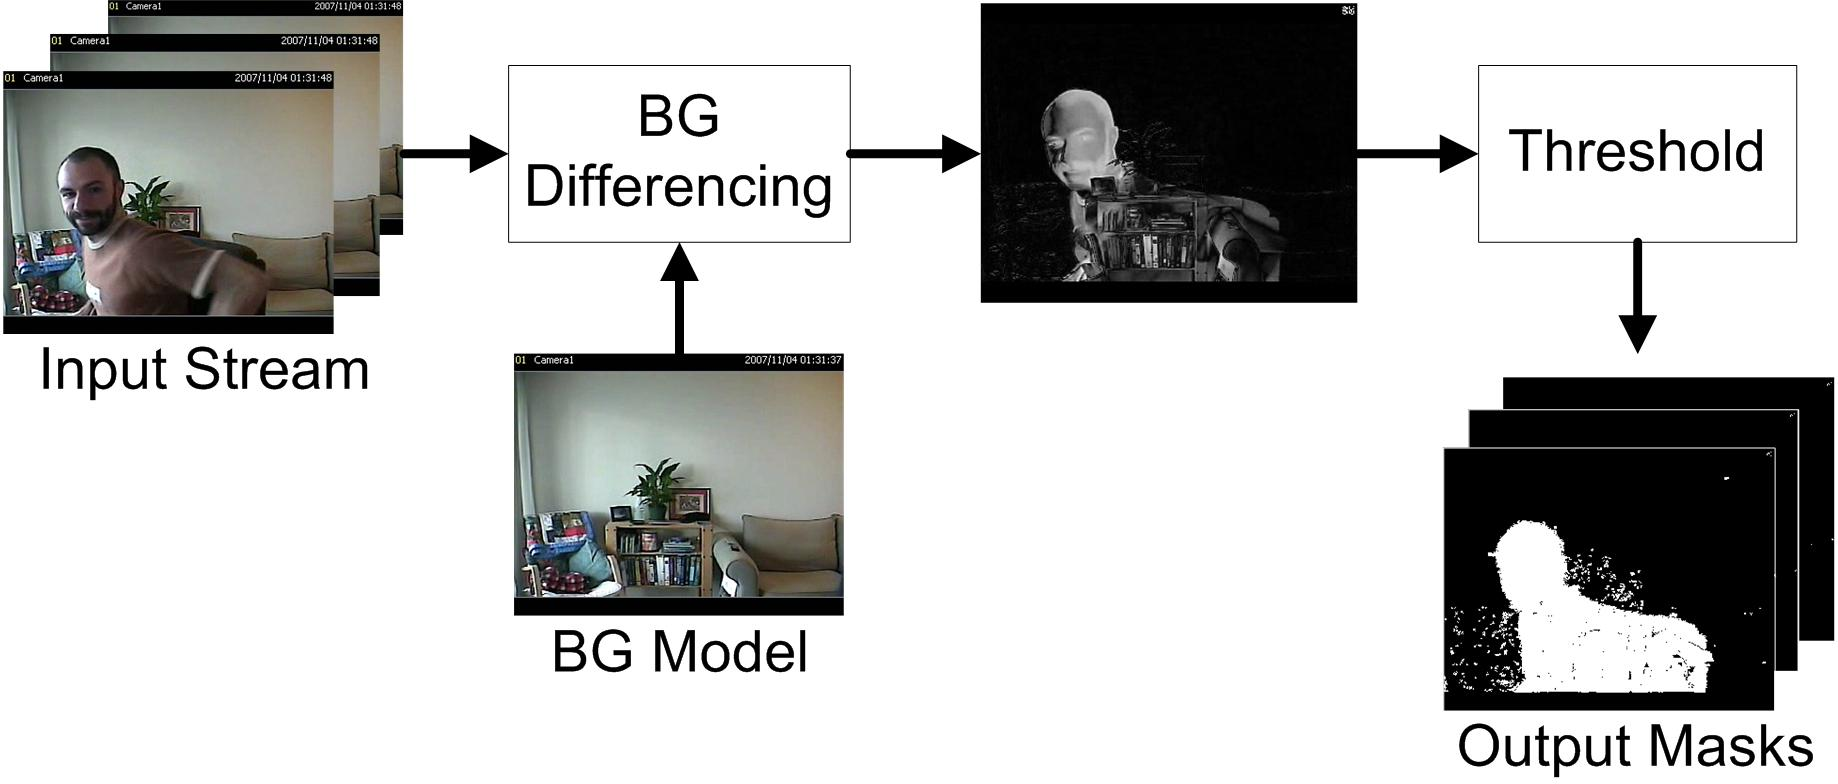
\includegraphics[scale=0.65]{BackgroundSegmentation}
	\caption{Voorbeeld voorgrond/achtergrond segmentatie}
	\label{imgVAS}
\end{figure}

Voorgrond/achtergrond segmentatie wordt vaak gebruikt in video surveillance \cite{bibBET3}. Deze techniek kan je splitsen in twee verschillende types namelijk recursief en niet recursief. Eerst bespreken we de recursieve technieken dit wordt gevolgd door de niet-recursieve technieken. Elk van deze technieken kan op verschillende manieren gebeuren. Elk van deze manieren heeft zijn voordelen en nadelen op vlak van geheugen, snelheid en moeilijkheid. De eerste stap van de deze techniek is het bepalen van de achtergrond. Dit kan op drie verschillende manieren gebeuren, namelijk per pixel per regio en per frame. \cite{bibBET4}.  Het bepalen  van de achtergrond gebeurt in de achtergrondmodelleringsfase. Deze techniek heeft 2 verschillende nadelen. Het eerste nadeel is dat hij licht gevoelig is, als je het licht aan doet, verandert het beeld. Hierdoor kunnen valse detecties optreden.  \cite{bibBET4}. Het tweede nadeel is dat de techniek gevoelig is voor de beweging van de camera. Je kan deze techniek dus enkel toepassen op beelden gefilmd met een statische camera \cite{bibBET7}. Als allerlaatste bespreken we een manier om voorgrond/achtergrond segmentatie toe te passen op thermische beelden \cite{bibBET5},\cite{bibBEt},\cite{bibBET2}. Vaak worden verschillende technieken gecombineerd om betere resultaten te krijgen. De meeste achtergrond segmentatie technieken  zijn niet in staat om tot goede resultaten te komen in aanwezigheid van ruis, verandering in licht en een niet statische achtergrond \cite{bibBET9}\\
Voorgrond/achtergrond segmentatie technieken moeten met 3 zaken rekeninghouden om succesvol te zijn
\begin{itemize}
	\item Wat is het model en hoe gedraagt het zich?
	\item Hoe wordt het model ge\"initialiseerd?
	\item Hoe wordt het model ge\"updatet?
\end{itemize}
\cite{bibBET8}


\subsubsection{Recursieve technieken}
\label{refRT}
Het achtergrond model wordt op recursieve wijze bij elke frame ge\"updatet. Dit wordt eveneens een adaptieve techniek genoemd.  Het voordeel hiervan is dat je geen extra frames moet bewaren in een buffer. Het nadeel hiervan is dat als er zich een fout voordoet in het achtergrond model dit ook voor lange tijd in het achtergrond model bewaard blijft. We bespreken vier verschillende recursieve methodes om de achtergrond te bepalen. De eerste techniek is running avarage,  de tweede is de approximated median filtering gevolgd door mixture of gaussian en om af te sluiten bespreken we $\Sigma$ - $\Delta$ achtergrond segmentatie.

\paragraph{Running avarage}
\label{refRUA}
Het achtergrond model wordt voor deze techniek bepaald aan de hand van volgende formule:
\begin{displaymath}
A_{i+1}=\alpha F_i+(1-\alpha)A_i
\end{displaymath}
met:
\begin{description}
	\item[A\textsubscript{i}] De huidige achtergrond
	\item[$\alpha$] De leersnelheid, vaak 0.05, met een waarde tussen 0 en 1
	\item[F\textsubscript{i}] De huidige frame
\end{description}
\cite{bibBEt}.Dit wilt zeggen dat het achtergrond model gemaakt wordt door voor elke pixel de gemiddelde waarde te nemen van de waarde in de vorige achtergrondschatting en de huidige framewaarde. De achtergrond gaat dus mee veranderen in de loop van de tijd. \\
Men kan de voorgaande formule generaliseren door het te schijven in incrementele vorm:
\begin{displaymath}
A_{i+1}=A_i+\delta_t F_i
\end{displaymath}
met:
\begin{description}
	\item[A\textsubscript{i}] De huidige achtergrond
	\item[$\delta_t$] increment fuctie, afhankelijk van de huidige frame
	\item[F\textsubscript{i}] De huidige frame
\end{description}
\cite{bibSDB}

De voordelen van deze methode zijn
\begin{itemize}
	\item Eenvoudige berekeningen
	\item Er wordt niet veel geheugen gevraagd
	\item De bepaling van de achtergrond gaat heel snel
	\item De methode is eenvoudig te implementeren.
	\item Houdt rekening met veranderingen in de achtergrond
\end{itemize}
De nadelen van deze methode zijn
\begin{itemize}
	\item Het resultaat is een schatting en is dus niet precies
	\item $\alpha$ moet geregeld worden om zo nauwkeurig mogelijke resultaten te krijgen.
	\item De nauwkeurigheid van de achtergrond schatting is afhankelijk van de snelheid waarmee het object door het beeld beweegt.
\end{itemize}
Er is ook een niet recursieve tegenhanger, deze noemt men exponential smoothing \cite{bibSDB}.


\paragraph{Approximated Median Filtering}
\label{refAMF}
Deze methode heeft ook een niet recursieve tegenhanger. Omdat ze zo'n goede resultaten opleveren en de berekening zeer eenvoudig is. Het principe is als volgt: als de grijswaarde van de pixel die men bekijkt groter is dan de grijswaarde van de geschatte achtergrond, wordt de grijswaarde van deze pixel in de geschatte achtergrond verhoogt met 1. Dezelfde redenatie voert men ook uit als de grijswaarde van de pixel kleiner is dan de grijswaarde van de overeenkomstige pixel in de geschatte achtergrond. Het achtergrond model zal dus mee aanpassen in de tijd. De waarden van de achtergrond gaan convergeren naar de effectieve mediaan. Hierdoor zal er steeds minder rekenwerk nodig zijn \cite{bibVTS}.\\
De voordelen van deze methode zijn:
\begin{itemize}
	\item Zeer eenvoudige implementatie
	\item Hoge nauwkeurigheid
	\item Niet veel geheugen nodig
	\item De techniek is robuust
\end{itemize} 
De nadelen van deze techniek zijn:
\begin{itemize}
	\item Als er een wijziging is in de achtergrond, past hij zich maar traag aan
\end{itemize}

\paragraph{Mixture of Gausian}
\label{refMOG}
Mixture of gausian ook wel MOG genoemd zal aan de hand van model bepalen of een pixel tot de voor- of achtergond hoort. Als de waarde van de pixel in de huidige frame hoort binnen de waarden van de achtergrond, zal deze tot de achtergrond gerekend worden. Het updaten van de achtergrond is afhankelijk van de waarschijnlijkheid van de waarden van het nieuwe frame. De waarden waarmee ge\"incrementeerd worden zijn eveneens afhankelijk van de dichtheid van de achtergrond. Als de dichtheid groter is, zal de incrementeer waarde ook groter zijn \cite{bibSDB}. \\
Voordelen van de methode:
\begin{itemize}
	\item Er is geen vaste drempelwaarde
	\item Deze methode is nauwkeuriger dan de running avarage en approximated median filtering methodes die eerder beschreven werden.
	\item Kan tegen lange termijn veranderingen en herhalende bewegingen.
\end{itemize}
Nadelen van deze methode:
\begin{itemize}
	\item Deze methode is traag.
	\item Veel moeilijke berekeningen nodig om de achtergrond te bepalen
\end{itemize}
De nadelen wegen zwaarder op dan de voordelen. Daardoor wordt deze techniek minder vaak gebruikt \cite{bibSDB}.

\paragraph{ $\Sigma$ - $\Delta$ achtergrond segmentatie}
De $\Sigma$ - $\Delta$ achtergrond segmentatie is een eenvoudige, niet lineaire methode om de achtergrond te bepalen \cite{bibSDB}. Het wordt vaak gebruikt in ingebedde toepassingen \cite{bibBET8}. Om de achtergrond te bepalen wordt aangenomen dat de achtergrond voor het grootste deel van de tijd zichtbaar is \cite{bibSDB2}. Het is gebaseerd op vergelijken en elementaire optellingen en verschillen. 
Door middel van een functie bepaalt men de waarschijnlijkheid van de waarde van de pixel van de volgende frame, dit noemt men het dichtheidsmodel .  Hoe hoger de waarschijnlijkheid van een pixel, hoe kleiner de nood om het te gaan updaten, hierdoor is de geschatte achtergrond stabieler. \cite{bibSDB2} Men gaat dan de pixelwaarde vergelijken met de waarde van het dichtheidsmodel en de waarde van de achtergrond aanpassen. Een mogelijke manier om de geschatte waarde te bepalen is door gebruik te maken van de Zipf law, dit is een hyperbolisch afnemende functie. Ook hier treedt het apperture probleem op, dit wilt zeggen dat de middelste delen van bewegende delen niet mee gedetecteerd worden. De relevantie van deze techniek is te vergelijken met die van MOG \cite{bibSDB}.\\
Voordelen van de methode:
\begin{itemize}
	\item Eenvoudig te berekenen
\end{itemize}


\subsubsection{Niet recursieve technieken}
\label{refNRT}
De niet-recursieve technieken maken gebruik van een sliding window benadering voor het bepalen van de achtergrond. De laatste frames worden opgeslagen in de buffer en de achtergrond wordt bepaald door temporele variatie van elke pixel. Het voordeel van deze methode is dat ook personen die lang in dezelfde houding op het bed liggen ook gedetecteerd worden. Het nadeel hiervan is dat de buffer een groot deel geheugen in beslag neemt. Er zijn verschillende methodes om het achtergrond model te bepalen. We bespreken er drie, als eerste bespreken we temporeel verschil, de tweede methode is temporeel verschil met drie frames, als laatste bespreken we median filter.

\paragraph{Temporeel verschil}
\label{refFRD}
Dit is een zeer eenvoudige model. Deze methode wordt gebruikt om bewegende objecten uit een reeks van afbeeldingen te halen. De gedetecteerde oppervlakken omvatten de doel oppervlakken en kleine oninteressante oppervlakken (bijvoorbeeld kleine veranderingen in de achtergrond) \cite{bibTeV}. Je neemt twee opeenvolgende frames, neemt daarna het verschil, dit verschil wordt dan vergeleken met een drempelwaarde. \cite{bibIPC2}. Aangezien een pati\"ent in zijn slaap heel weinig gaat bewegen, is dit voor ons geen goede methode. Hoe weet anders het systeem of de persoon stil in bed ligt of hij uit het beeld verdwenen is? Een nadeel van deze techniek is dat men gebruik maakt van een sequentie van beelden en dat de detectie dus een paar frames later gebeurt. \cite{bibIRC}. De techniek kan zeer goed tegen dynamische veranderingen van de omgeving. Maar geeft niet alle relevante pixels als oplossing, er ontstaan gaten in bewegende objecten. \cite{bibTVD}.
\begin{displaymath}
|frame_{i}-frame_{i-1}|>T
\end{displaymath}
met
\begin{description}
	\item [frame\textsubscript{i}] het huidige frame
	\item [frame\textsubscript{i-1}] het vorige frame
	\item [T] de drempelwaarde
\end{description}
Als het verschil groter is dan de drempelwaarde, dan hoort die pixel bij de voorgrond. \cite{bibBET3}. De drempelwaarde wordt empirisch bepaald.\\
Voordelen:
\begin{itemize}
	\item Weinig rekenkracht nodig.
	\item De methode is zeer adaptief.
	\item Er wordt zeer weinig extra geheugen gebruikt.
	\item Het model wordt snel bijgewerkt als er iets verandert in de achtergrond.
\end{itemize}
Nadelen:
\begin{itemize}
	\item Als een persoon niet beweegt, verdwijnt deze mee in de achtergrond.
	\item Als een object een gelijkmatig verdeelde intensiteit waarden heeft, de middelste delen mee verdwijnen in de achtergrond
	\item Deze methode is zeer gevoelig voor ruis.
	\item Het is moeilijk om de juiste drempelwaarde te vinden.
	\item Een kleine verandering in de achtergrond wordt mee als voorgrond gezien 
\end{itemize}
\cite{bibTeV}

\paragraph{Temporeel verschil met drie frames}
Deze methode is een uitbereiding op de methode die we in de vorige paragraaf hebben besproken. Het grootste verschil is dat er drie opeenvolgende frames gebruikt worden om de achtergrond te berekenen. Het blok diagram van deze methode vindt u in figuur \ref{imgTeV}. 
Zoals u in de figuur kan zien, zijn er verschillende stappen in het algoritme. Hieronder gaan we ze stap voor stap uitleggen.
\begin{figure}[h]
	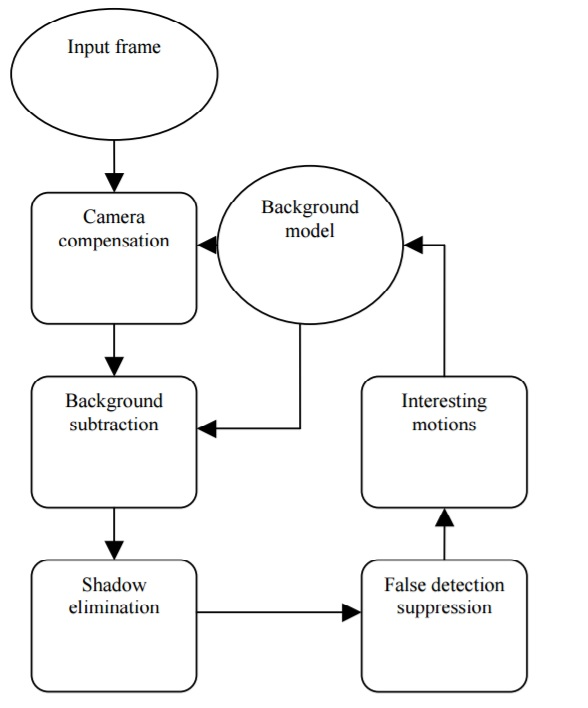
\includegraphics[scale=0.6]{TemporeelVerschilDrieFrames}
	\caption{Blokschema temporeel verschil van drie Frames}
	\label{imgTeV}
\end{figure}

\subparagraph{Camera compensatie}
Hier worden eventuele kleine bewegingen van de camera gecompenseerd, omdat temporeel verschil heel gevoelig is aan kleine veranderingen in het beeld. Dit gebeurt door middel van een algoritme dat enkele standaard pixels in het frame neemt en vervolgens de beweging schat door middel van een matching methode. Vervolgens wordt het volledige inputframe aangepast.  Indien je werkt met een statische camera hoef je deze stap niet te doen.

\subparagraph{Temporeel verschil door middel van drie frames}
Vervolgens wordt het temporeel verschil gebruikt om snel de bewegende objecten uit het input beeld te halen. De drie frames worden verdeeld in twee groepen. De eerste groep bevat de twee voorgaande frames, de tweede groep bevat de input frame en het voorgaande frame. Van deze twee groepen wordt dan het temporeel verschil zoals besproken in de voorgaande paragraaf berekend. Vervolgens kan men door de intersectie te nemen van de twee berekende verschillen eenvoudig de beweging berekenen van het vorige frame, deze komt namelijk in de twee berekeningen voor. Vervolgens neemt men het verschil van het temporeel verschil van de tweede groep en de juist berekende intersectie. Nu houd je de bewegende delen over van het laatste frame.

\subparagraph{Overige stappen}
De stappen na de berekening van het temporeel verschil worden gebruikt om de twee problemen die optreden door het gebruikt van de methode ongedaan te maken. De eerste is dat het onmogelijk is om altijd het volledig bewegende object te detecteren, dit doordat er kleine gaten ontstaan in het bewegend object door de berekening van het temporeel verschil. Het tweede is dat deze techniek heel gevoelig is voor kleine veranderingen en er dus ook oninteressante regio's zijn die gedetecteerd worden \cite{bibTeV}.

\paragraph{Median Filter}
\label{refMEF}
Deze techniek wordt zeer vaak toegepast. Hij zegt dat de mediaan van elke pixel van de n laatste  frames in de buffer de achtergrond is. De redenatie hierachter is dat de achtergrond in de helft van de frames ongewijzigd gaat blijven.\\
Voordelen:
\begin{itemize}
	\item Weinig rekenkracht voor nodig.
	\item Levert vrij nauwkeurige resultaten.
\end{itemize}
De nadelen van deze methode zijn
\begin{itemize}
	\item Vrij veel geheugen capaciteit nodig.
\end{itemize}


\subsubsection{Per pixel proces}
\label{refPPP}
Men kijkt naar elk pixel signaal als een onafhankelijk proces. Deze methode wordt tegenwoordig het meeste gebruikt omdat men hiervoor weinig rekenkundige kracht nodig heeft. Al de methodes die hierboven besproken werden zijn per pixel processen. Het principe is zeer eenvoudig. Men vergelijkt de achtergrond pixel per pixel met de huidige frame. Bij het gebruiken van deze techniek, wordt er eveneens vanuit gegaan dat er een ruimtelijke consistentie is. Dit kan resulteren in lokale mis classificaties \cite{bibBET8}.

\subsubsection{Per regio proces}
\label{refPRP}
Men gaat de regio rond de pixel mee bekijken. Dit wordt gedaan om valse positieve signalen te minimaliseren. Deze methode levert een robuustere versie op van het model. Men neemt aan dat de omgeving van een pixel ook tot het zelfde object in de achtergrond hoort. Er wordt ook vanuit gegaan dat als de waarde van een pixel verandert, er soortgelijke veranderingen optreden in de aanliggende pixels. Daarom vergelijkt men de ogenblikkelijke pixel waarde met de waarden van de omgeving in de achtergrond. Deze methode zorgt wel voor problemen bij pixels waarvan de omgeving op de rand ligt met meerdere achtergrond object  \cite{bibBET8}.

\subsubsection{Per frame proces}
\label{refPFP}
Bij deze methode kijkt men naar het gehele frame. Dit wordt gebruikt om bijvoorbeeld de gevoeligheid voor het aandoen van het licht te verkleinen. Men gebruikt deze techniek om plotse en globale veranderingen te detecteren \cite{bibBET8}.

\subsubsection{Voorgrond/Achtergrond segmentatie voor thermische beelden}
\label{refBETB}
Door de kringen die optreden rond de personen in thermische beelden, zijn de klassieke methoden voor voorgrond/achtergrondsegmentatie hier niet van toepassing. Deze methode steunt niet op vorige vorm modellen of bewegingsinformatie. Het algoritme werkt in drie stappen, het eerste is het bepalen van een interessante regio, het tweede is de contour detectie, als laatste wordt de contour gesloten \cite{bibBET5}. De beste resultaten voor persoonsdetectie in thermische beelden gebeurt door gebruik te maken van trainbare, klasse specifieke object detectors \cite{bibBET7}.

\paragraph{Regio detectie}
We zoeken interessante regio's (ROI) die de personen en hun halo bevatten. Hiervoor kunnen verschillende technieken gebruikt worden zoals  het standaard gausisch model dat eerder besproken werd en een standaard intensiteit gebaseerde statistische achtergrond segmentatie techniek \cite{bibBET6}. Om de ROI uit de beelden te halen wordt er gebruik gemaakt van een 5x5 dillatie, gevolgd door een algoritme om de aaneengesloten componenten te extraheren. Als de ROI te klein is wordt het automatisch weer verwijderd \cite{bibBET5}.

\paragraph{Contour detectie}
We bekijken elke ROI individueel , zodat we de persoon van zijn halo kunnen scheiden. Op elke regio wordt een Contour Saliency Map (CSM) toegepast. De waarde van elke pixel in de CSM bepaalt of de pixel behoort tot de persoon of de omgeving. Een CSM wordt bepaald door een vermenigvuldiging van de genormaliseerde voorgrond gradi\"ent magnitudes met de genormaliseerde voorgrond-achtergrond gradi\"ent verschillen magnitude in de ROI. Vervolgens gaan we de representatie van de CSM verkleinen, vervolgens wordt er een threshold toegepast om de beste pixels te selecteren. Daarna gaan we terug kijken naar de ROI's als het een zeer warm persoon was, gaat de detectie die we net gedaan hebben in de kring vallen, dan wordt het contour sterker getekend \cite{bibBET5}.

\paragraph{Contour sluiten}
De oplossing van de contour detectie is open. In de laatste stap wordt de contour aangevuld door per pixel te zoeken waar de dichtstbijzijnde contourpixels zijn \cite{bibBET5}.

\subsection{Vormgebaseerde benadering}
\label{refVBB}
Deze techniek tracht de problemen die optreden bij het herkennen van de pati\"ent op de lossen. Zoals het verdwijnen van een pati\"ent die zeer stil ligt of het ontstaan van geesten (personen die gedetecteerd worden maar er niet effectief zijn.) Het grootste probleem voor deze techniek is dat pati\"enten in veel verschillende vormen kunnen voorkomen \cite{bibIRC}. Dit ligt bijvoorbeeld aan slaaphouding en/of lichaamsbouw. Dit kan men oplossen door personen op te delen in de verschillende lichaamsdelen. Dit is op zichzelf al een zeer moeilijke taak.  
Het principe is zeer eenvoudig, als eerste wordt er een template in de vorm van een persoon ingeladen. Dan wordt de template over de afbeelding geschoven terwijl er gezocht wordt naar een overeenkomst \cite{bibIRC4}.

\section{Besluiten uit de literatuurstudie}
\label{refLBe}